\documentclass[12pt,a4paper]{article}

\usepackage[utf8]{inputenc}
\usepackage[T1]{fontenc}
\usepackage[english]{babel}
\usepackage{amsmath}
\usepackage{ae}
\usepackage{units}
\usepackage{icomma}
\usepackage{color}
\usepackage{graphicx}
\usepackage{bbm}
\newcommand{\N}{\ensuremath{\mathbbm{N}}}
\newcommand{\Z}{\ensuremath{\mathbbm{Z}}}
\newcommand{\Q}{\ensuremath{\mathbbm{Q}}}
\newcommand{\R}{\ensuremath{\mathbbm{R}}}
\newcommand{\C}{\ensuremath{\mathbbm{C}}}
\newcommand{\rd}{\ensuremath{\mathrm{d}}}
\newcommand{\id}{\ensuremath{\,\rd}}


\begin{document}

\title{Simulations of road blockages, Simulation of complex systems}
\author{Fredrik, Daniel, Thorben, Atonderski}
\date{\today}
\maketitle

\begin{abstract}
apaIn real-world traffic small errors, like an unnecessary brake from individual drivers can propagate through traffic and lead to interruptions and traffic jams far away from the initial disturbance. Studying these phenomena could be especially important with the emergence of self-driving cars. The cars need to be tuned so they don't cause unnecessary traffic congestion.

We want to study how small irregularites, such as braking or acceleration of a few drivers, in traffic flow propagate through traffic. We start from a single lane situation with agent-based modelling of individual drivers and periodic boundary condidtions. Each agent is represented by a finite-state machine with threes states, braking, acceleration and driving at constant speed. The state transitions depend on the speed and positions of the nearest neighbours, primarily the one ahead. Depending on the time available, more complexity will be added to the model.  

main features to be implemented:
Graphics - matplotlib/pygame,
Track - linked list, keep track of length, be able to give info to car.
Car - properties: speed, positions, (lane?), state (braking, acceleration, constant), (size?). Functions: update(), query track.
Braking - instantly
Crashes, not in the beginning
Main controller


\end{abstract}

\newpage
\tableofcontents
\newpage

\section{So far, i.e. predraft}
So far we've implemented a rudimentary model of the car track, with regular and more aggressive drivers and a visualization. We have also started implementing a basic density plot in order to see the propagation and or creation and dissipation of traffic congestions on the track. So far we have observed wave-like behaviour of car/speeds. Further work will concentrate on extending the model to multi-lane, and extracting the wave propagation-speed/amplitudes etc and their dependence on the number of drivers on the track and the ratio of normal/aggressive drivers and number of lanes etc.

\section{Introduction}
In real-world traffic small localized perturbations, like an unnecessary brake from an individual driver, can cause long-lasting interruptions and congestions in traffic flow for a long time after the initial disturbance \cite{kerner97flow}. The occuring sections of slow-moving flow can propagate through traffic and give rise to traffic jams involving cars far away from the disturbance \cite{kerner96trafficjam}.

https://en.wikipedia.org/wiki/Three-phase\_traffic\_theory

B.S Kerner As found in experimental data from real 

We explore how traffic jams can occur in a model of traffic flow on a three-lane highway and how different behaviour and actions of individual drivers give rise to congestions.

A characteristic measure of real-world traffic jams that can be used to verify the authenticity has been proposed by B.S Kerner \cite{kerner96trafficjam}. The characteristics include the density of vehicles in the traffic jam, the average velocity of the cars and the flow of traffic out from the jam.

Similar results as seen in experimental data
Bla bla

Write some about the negative aspects, cost, time, environment (accidents). Write some about potential causes.

Write what we want to explore.

Write a bit about self-driving cars.



\section{The model}
To model traffic behaviour we use an agent-based approach with each agent representing a car and the behaviour of its driver. The goal of each agent is to try to keep its set target speed on the track and avoid having to slow down. Different agents can have different personalities, some drivers are more aggressive while others try to drive more carefully to ensure not to disturb other drivers in traffic.

\subsection{The track}\label{track}
The track carries the main information of the simulation. It contains track length, number of lanes and a list of all cars on the track. The updating is mainly controlled by the track class.  \\
During one step in time, the track class communicates with every car to give information of nearest neighbours and the current speed limit. The car's behaviour is then controlled by the car class itself (see \ref{cars}). The track stores the updated information about the cars and checks the periodic boundary conditions. \\

% Not sure if we want to go into details about the implementation. Cut this out if we don't want it :)
In order for the model to scale to a large number of cars (at least 1000) the track needed to utilize an efficient data structure. The naive implementation of just storing all the cars in a list and iterating over that list proved to be too slow. If N is the number of cars the naive approach had a time complexity of at least O(N^2). A better approach was instead to divide the track into a lot of smaller pieces, "buckets". The buckets in turn stored a list of all the cars inside it. The bucket division was based on the position on the track, so that a given position mapped uniquely to a single bucket. The primary improvement came from the fact that given a certain car it was possible to directly look up all the cars in the same bucket, without having to consider any of the other buckets. The performance improved to close to O(N) instead of O(N^2), which made a big difference when N was approaching 1000 cars. Note that this new model collapses to the naive implementation if the number of buckets is 1.

\subsection{The cars} \label{cars}
The model contains three different car types: neutral drivers, passive drivers and aggressive drivers. The neutral driver is the mother class. Its attributes are position, velocity, acceleration and deceleration capability, length and a safety multiplier that affects the safety distance a car wants to hold. \\
All these attributes are also inherited by the other car classes. For the aggressive drivers and passive drivers the target speed, the acceleration and deceleration capability and the safety multiplier are manipulated by a factor of aggressiveness (> 1) or passiveness (<1). The safety multiplier is divided by this factor so that an aggressive driver tends to hold less distance and a passive driver holds more distance to cars in front. \\
During a step in time every car gets information from the track (\ref{track}) about its nearest neighbours and the allowed speed. Depending on the distance and speed to the car in front and the car behind the agent decides whether he needs to brake, can accelerate or needs to switch lanes to overtake. \\
For the lane switching behaviour two different possibilities are implemented, depending on the parameter: nice. If nice is set to be False, lanes are switched in two cases: when the agent is below its personal speed limit and can go faster on another lane or when a car behind is too close and faster.\\
If nice is set to be True, cars will try to drive as far right as possible. If the lane to the right is free and they do not have to reduce their velocity, nice cars will switch to that lane. 

\subsection{Initialisation}

\subsection{Observation}

%The agents are placed on a track of fixed length, but with periodic boundary conditions creating an infinite loop. Driving is only allowed in one direction, but to allow for more complexity and further model highway traffic the track can be extended to allow multiple parallel lanes with lane switching allowed. To decide on its actions each agent can see agents in its proximity, both in its lane and in other lanes bordering its own. The agent can read the velocity and position of these nearby agents to adjust its acceleration or decide to shift lanes.

\section{Results}

% Amount of slowdown during traffic jam for varying percentages of aggressive drivers
% Amount of slowdown during traffic jam for varying percentages of passive drivers (no improvement)
% Time vs average velocity for different safety distances
% Plot that shows how the bucket with the largest car concentration moves
% Still picture of the cars during a traffic jam
% (very very optional) nice vs normal cars

A basic example of the emergence of waves can be seen in figure \ref{fig:a3lanes} and \ref{fig:b3lanes}. Traffic starts in the rightmost lane and when traffic gets to dense cars starts shifting lanes. When more dense regions start to form cars spread out evenly between the lanes with clusters of cars going slower, congestion. These congestions travel through traffic like a wave, with new cars slowing down behind the congestion and getting stuck in it.
We can observe how a number of agressive drivers can increase the traffic flow by disrupting congestions. However, using only agressive drivers appears to reduce traffic flow in same manner as having only passive drivers. From this we conclude that there should be an optimal ratio of agressive drivers per passive drivers to maximize traffic flow. This result can be seen in figure \ref{jam_flow} where we have plotted traffic flow against the ratio of agressive drivers per passive drivers.

\begin{figure}[h]
    \centering
    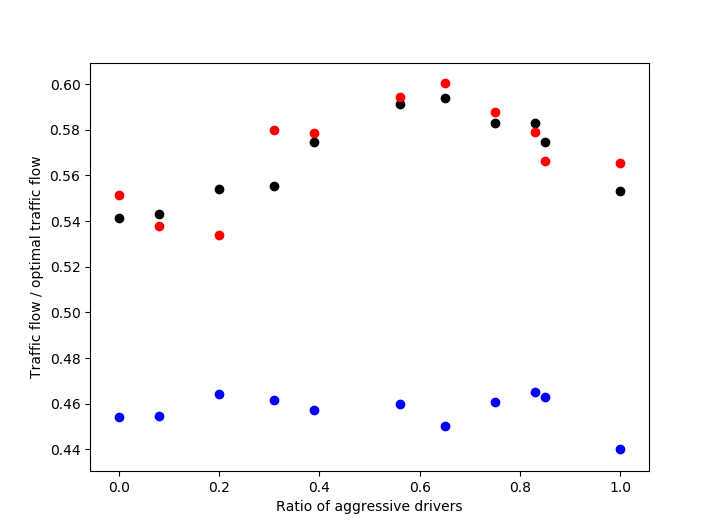
\includegraphics[scale=0.3]{figs/jam_flow_aggresives_150.png}
    \caption{Visualization of a three lane track with 500 cars. All cars started in the right-most lane but when traffic become too congested and cars can not keep their desired speed they switch lanes. Each lane is 1000 meters long. The cars are concentrated in the rightmost lane, but have started to migrate to the other lanes.}
    \label{fig:jam_flow}
\end{figure}

\begin{figure}[h]
    \centering
    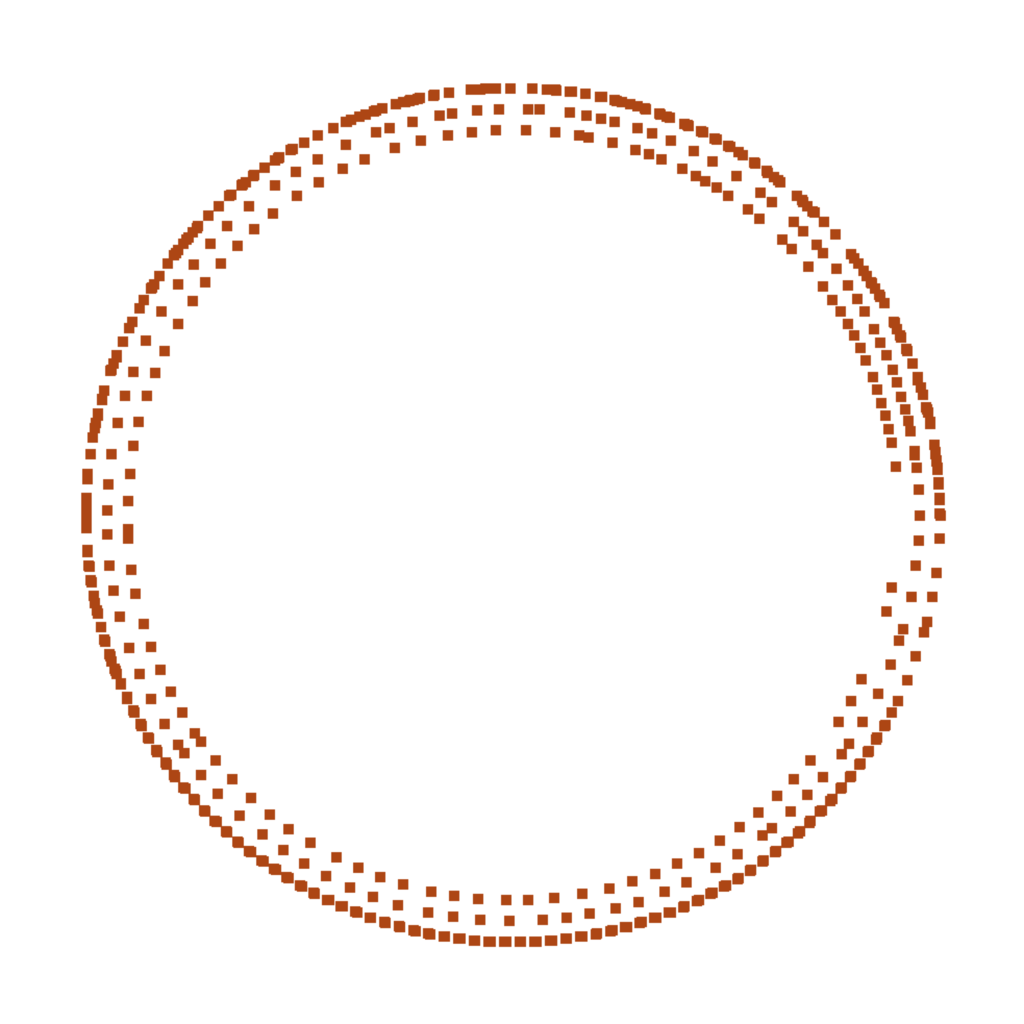
\includegraphics[scale=0.3]{figs/circular_three_lane.png}
    \caption{Visualization of a three lane track with 500 cars. All cars started in the right-most lane but when traffic become too congested and cars can not keep their desired speed they switch lanes. Each lane is 1000 meters long. The cars are concentrated in the rightmost lane, but have started to migrate to the other lanes.}
    \label{fig:a3lanes}
\end{figure}

\begin{figure}[h]     
    \centering
      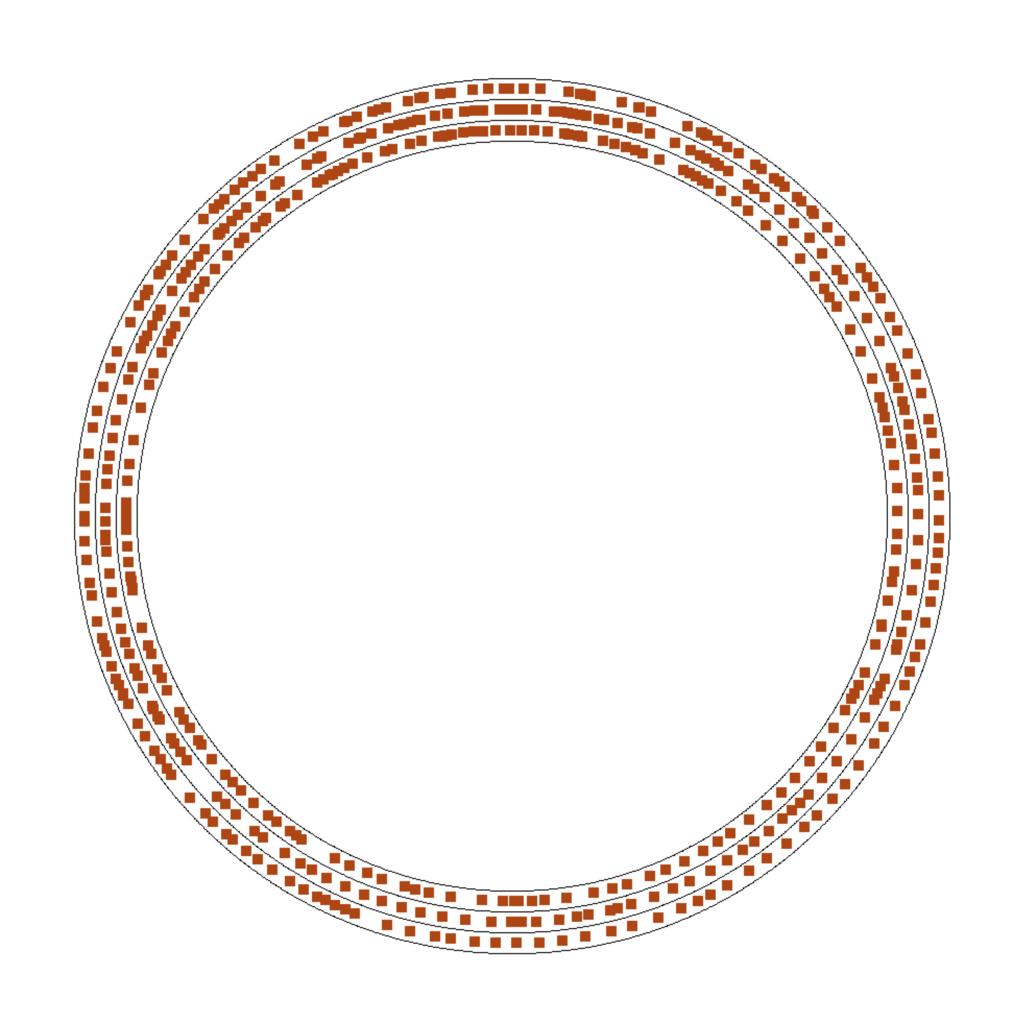
\includegraphics[scale=0.3]{figs/good_circular_three_lane.png}
      \caption{Congestions have started to form. These congestion clusters have cars moving slower than the rest. Congestions are propagated through traffic with new slow cars getting added from behind.}
      \label{fig:b3lanes}
\end{figure}



%\section{Parameter dependence of cluster formations etc...}

%\subsection{}

% Figurer inkluderade som eps-filer
%% \begin{figure}\centering
%% \includegraphics{filnamn.eps}
%% \caption{\label{figuren} Perioden $T$ som funktion av pendellängden.}
%% \end{figure}

% Figurer inkluderade med xfigs postscript+latex
%% \begin{figure}\centering
%% \input{filnamn.pstex_t}
%% \caption{\label{finafiguren} Perioden $T$ som funktion av
%%   pendellängden.}
%% \end{figure}
\bibliographystyle{unsrt}
\bibliography{bibliography}

\end{document}
